%% ESTA PARTE ES PARA EXPLICAR EL TURLTLEBOT3
\section{Managing a real robot: TurtleBot 3}%http://wiki.ros.org/Robots/TurtleBot

\begin{frame}{TurtleBot3}
\begin{itemize}
 \item TurtleBot is a ROS standard platform robot.
 \item There are 3 versions of the TurtleBot series. 
  \begin{enumerate}
   \item TurtleBot1 was developed by Tully (Platform Manager at Open Robotics) and Melonee (CEO of Fetch Robotics) from Willow Garage on top of the iRobot’s Roomba-based research robot, Create, for ROS deployment. It was developed in 2010 and has been on sale since 2011. 
   \item In 2012, TurtleBot2 was developed by Yujin Robot based on the research robot, iClebo Kobuki. 
   \item In 2017, TurtleBot3 was developed with features to supplement the lacking functions of its predecessors, and the demands of users. The TurtleBot3 adopts ROBOTIS smart actuator Dynamixel for driving.
  \end{enumerate}   
 \item TurtleBot3 is a small, affordable, programmable, ROS-based mobile robot for use in education, research, hobby, and product prototyping.
 \item TurtleBot3 is a collaboration project among Open Robotics, ROBOTIS, and more partners.
\end{itemize}
\begin{block}{TurtleBot3 Introduction Video}
\url{https://youtu.be/9OC3J53RUsk}
\end{block}
\end{frame}

\subsection{Turtlebot Installation}

\begin{frame}[fragile, allowframebreaks]{PC installation}
Install ROS on Remote PC:
\begin{lstlisting}[language=shell]
$ sudo apt update
$ sudo apt upgrade
$ wget https://raw.githubusercontent.com/ROBOTIS-GIT/robotis_tools/master/install_ros_noetic.sh
$ chmod 755 ./install_ros_noetic.sh 
$ bash ./install_ros_noetic.sh
\end{lstlisting}

Install Dependent ROS Packages:
\begin{lstlisting}[language=shell]
$ sudo apt-get install ros-noetic-joy ros-noetic-teleop-twist-joy ros-noetic-teleop-twist-keyboard ros-noetic-laser-proc ros-noetic-rgbd-launch ros-noetic-rosserial-arduino ros-noetic-rosserial-python ros-noetic-rosserial-client ros-noetic-rosserial-msgs ros-noetic-amcl ros-noetic-map-server ros-noetic-move-base ros-noetic-urdf ros-noetic-xacro ros-noetic-compressed-image-transport ros-noetic-rqt* ros-noetic-rviz ros-noetic-gmapping ros-noetic-navigation ros-noetic-interactive-markers ros-noetic-turtlebot3-msgs ros-noetic-turtlebot3-description ros-noetic-dynamixel-sdk ros-noetic-turtlebot3
$ cd ~/catkin_ws && catkin_make
\end{lstlisting}

Network configuration. Add the following lines to your $\sim$/.bashrc file:
\begin{lstlisting}[language=shell]
export TURTLEBOT3_MODEL=burger
export ROS_MASTER_URI=http://localhost:11311
export ROS_HOSTNAME=localhost
\end{lstlisting}
Usually, ROS\_MASTER\_URI and ROS\_HOSTNAME doesn't look like this. An usual configuration would be like this:
\begin{figure}
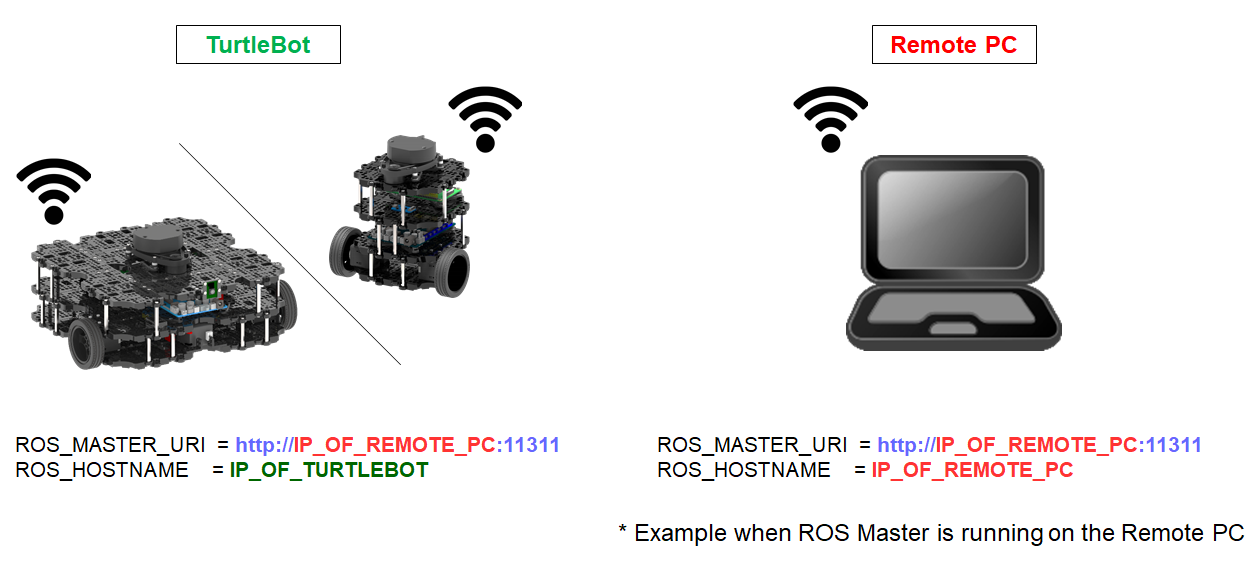
\includegraphics[width=.65\textwidth]{./img/ros/network_configuration.png}
\end{figure}
\end{frame}

\begin{frame}{TurtleBotPC and OpenCR installation}
To finish your installation you also need to:
\begin{itemize}
 \item Install Linux, ROS and hardware related packages to control the TurtleBot3 on your TurtleBot PC.
  \begin{itemize}
   \item \url{http://emanual.robotis.com/docs/en/platform/turtlebot3/sbc_setup/}
  \end{itemize}
  \begin{figure}
   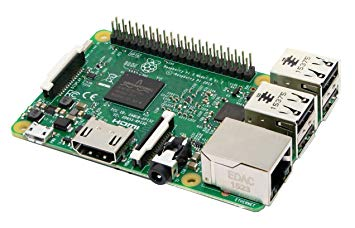
\includegraphics[height=1.7cm]{./img/ros/raspberry.jpg}
  \end{figure}
 \item Upload latest firmware of TurtleBot3 to embedded board OpenCR.
  \begin{itemize}
   \item \url{http://emanual.robotis.com/docs/en/platform/turtlebot3/hardware_setup/}
  \end{itemize}
  \begin{figure}
   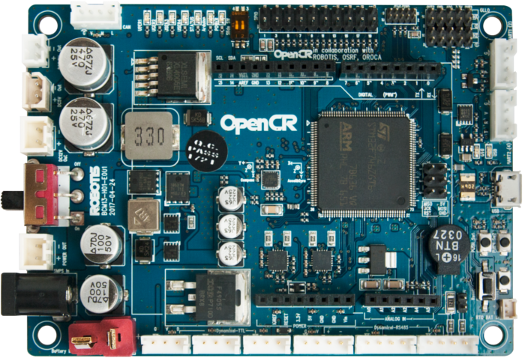
\includegraphics[height=1.7cm]{./img/ros/opencr.png}
  \end{figure}
\end{itemize}
\end{frame}

\subsection{Turtlebot Simulation}

\begin{frame}[fragile]{TurtleBot3 Simulation Installation}

\begin{lstlisting}[language=shell]
$ sudo apt-get install ros-noetic-joy ros-noetic-teleop-twist-joy ros-noetic-teleop-twist-keyboard ros-noetic-laser-proc ros-noetic-rgbd-launch ros-noetic-rosserial-arduino ros-noetic-rosserial-python ros-noetic-rosserial-client ros-noetic-rosserial-msgs ros-noetic-amcl ros-noetic-map-server ros-noetic-move-base ros-noetic-urdf ros-noetic-xacro ros-noetic-compressed-image-transport ros-noetic-rqt* ros-noetic-rviz ros-noetic-gmapping ros-noetic-navigation ros-noetic-interactive-markers ros-noetic-turtlebot3-msgs ros-noetic-turtlebot3-description
$ export TURTLEBOT3_MODEL=burger
$ cd ~/catkin_ws/src/
$ git clone -b noetic-devel https://github.com/ROBOTIS-GIT/turtlebot3_simulations.git
$ cd ~/catkin_ws && catkin_make
\end{lstlisting}

% The turtlebot3\_simulation metapackage requires turtlebot3 metapackage and turtlebot3\_msgs package as a prerequisite. 

% \vspace{.1cm}
% The turtlebot3\_fake is a very simple simulation node that can be run without having an actual robot. To launch the virtual robot, execute the turtlebot3\_fake.launch file in the turtlebot3\_fake package:
% \begin{lstlisting}[language=shell]
% $ roslaunch turtlebot3_fake turtlebot3_fake.launch
% \end{lstlisting}

% You can even control the virtual TurtleBot3 in RViz with a teleoperation node.
% \begin{lstlisting}[language=shell]
% $ roslaunch turtlebot3_teleop turtlebot3_teleop_key.launch
% \end{lstlisting}
\end{frame}

\begin{frame}[fragile]{TurtleBot3 Simulation using Gazebo}
The following command can be used to test the virtual TurtleBot3 on the empty world of the gazebo default environment.
\begin{lstlisting}[language=shell]
$ roslaunch turtlebot3_gazebo turtlebot3_empty_world.launch
\end{lstlisting}

TurtleBot3 world is a map consists of simple objects that makes up the shape of TurtleBot3 symbol. TurtleBot3 world is mainly used for testing such as SLAM and Navigation.  
\begin{lstlisting}[language=shell]
$ roslaunch turtlebot3_gazebo turtlebot3_world.launch
\end{lstlisting}

TurtleBot3 House is a map made with house drawings. It is suitable for testing related to more complex task performance.
\begin{lstlisting}[language=shell]
$ roslaunch turtlebot3_gazebo turtlebot3_house.launch
\end{lstlisting}

In order to control a TurtleBot3 with a keyboard, launch teleoperation feature with below command in a new terminal window.
\begin{lstlisting}[language=shell]
$ roslaunch turtlebot3_teleop turtlebot3_teleop_key.launch
\end{lstlisting}

RViz visualizes published topics while simulation is running. 
\begin{lstlisting}[language=shell]
$ roslaunch turtlebot3_gazebo turtlebot3_gazebo_rviz.launch
\end{lstlisting}
\end{frame}